\documentclass[a4paper,11pt]{article}
\usepackage{fancyhdr}
\usepackage{graphicx}
\usepackage{url}
\usepackage{breakurl}
\usepackage[breaklinks]{hyperref}

\def\UrlBreaks{\do\/\do-}

\begin{document}
\pagestyle{fancy}
\fancyhead[L]{120001757}
\fancyhead[C]{CS3302-DE P2}
\fancyhead[R]{\today}
\fancyfoot[C]{\thepage}

\section{Implementation}
    All specified functionality has been implemented as required, and may be run as documented below.

    The program may be run in \textit{optimise} mode by passing the `-optimise' flag as well as parameters specifying the error probability (`-p') and maximum proportion of data bits which may be corrupted (`-maxCorruption'). The optimum value for \textit{r} will be calculated algorithmically and printed out along with the information rate and predicted proportion of data bits which will be corrupted on average. Example command:
\begin{verbatim}
    $ java -jar error-correction.jar -optimise -p 0.01
      -maxCorruption 0.005
\end{verbatim}

    When running in \textit{encode} mode (`-encode') an error probability (`-p'), value for r (`-r') and length of input data to generate (`-length') can be passed. Random data of the specified length (rounding down to the nearest multiple of data length) will be generated, encoded using the Hamming code of specified length, passed through a noisy channel with specified error probability and decoded using the same Hamming code. The proportion of bits corrupted in this process will be printed, along with the algorithmic prediction for comparison. Example command:
\begin{verbatim}
    $ java -jar error-correction.jar -encode -p 0.01 -r 5
      -length 100000
\end{verbatim}

    \subsection{Corruption Prediction}
        Several different methods of calculating the prediction for corruption proportion were implemented, initially starting with a simple formula of $p_{err} = 1 - (P(0) + P(1))$ where $P(x)$ is the probability of $x$ bits in a code word being corrupted after passing through the noisy channel. After further thought, this was realised to actually be a calculation for the proportion of corrupted blocks, so a new formula was required.

        The second formula implemented was a much more sophisticated binomial expansion, calculating the sum of all probabilities of potential corruptions from 2 to $n$ bits, with each portion being multiplied by the fraction of the input code word which would be corrupted after correction. The numerator of this fraction is always a multiple of three, as this is the minimum distance of a Hamming code. This method was very accurate for small values of $r$, but caused overflow errors as the length of code words increases extremely quickly.

        The final formula uses an approximation, calculating the average proportion of blocks that will be corrupted, and then multiplying this by the average number of bits that will be corrupted in any given block for the given p (it is given that the block is corrupted after correction, meaning that at least 3 bits will be corrupted). This formula has proved extremely accurate, as shown in tables \ref{table:r2}, \ref{table:r5} and \ref{table:r12} below. All data for these tables was generated using the `-benchPredict' flag.

        Note: the value of $r$ has been bounded to a maximum of 12, as beyond this point is not only very slow to calculate, but also begins to cause heap overflow errors at runtime.

        \begin{table}
        \centering
            \caption {r = 2}
            \label{table:r2}
            \begin{tabular}{l|llll}
            p    & predicted  & actual     & \% diff     \\\hline
            0.001 & 0.000003   & 0.00000338 & 11.24260355 \\
            0.005 & 0.00007475 & 0.00008375 & 10.74626866 \\
            0.01  & 0.000298   & 0.000289   & 3.11418685  \\
            0.02  & 0.001184   & 0.001176   & 0.68027211  \\
            0.03  & 0.002646   & 0.00266713 & 0.79223735  \\
            0.04  & 0.004672   & 0.00468375 & 0.25086736  \\
            0.05  & 0.00725    & 0.00725888 & 0.12233292  \\
            0.1   & 0.028      & 0.02790475 & 0.34133974  \\
            0.2   & 0.104      & 0.10391188 & 0.08480262  \\
            0.5   & 0.5        & 0.50023975 & 0.04792702  \\\hline
            ~     & ~          & avg        & 2.74228382  \\
            \end{tabular}
        \end{table}

        \begin{table}
        \centering
            \caption {r = 5}
            \label{table:r5}
            \begin{tabular}{l|lll}
             p    & predicted  & actual     & \% diff     \\ \hline
            0.001 & 0.00004414 & 0.00004238 & 4.15290231  \\
            0.005 & 0.00102176 & 0.00102138 & 0.03720457  \\
            0.01  & 0.00371511 & 0.00383925 & 3.23344403  \\
            0.02  & 0.01231211 & 0.01305751 & 5.70859222  \\
            0.03  & 0.02304064 & 0.02545915 & 9.49957088  \\
            0.04  & 0.03421095 & 0.03931479 & 12.98198464 \\
            0.05  & 0.04484546 & 0.05332343 & 15.89914602 \\
            0.1   & 0.08036471 & 0.11805787 & 31.92769783 \\
            0.2   & 0.19187118 & 0.21871134 & 12.27195627 \\
            0.5   & 0.48387096 & 0.50017975 & 3.26058582  \\ \hline
            ~     & ~          & ~          & 9.89730846  \\
            \end{tabular}
        \end{table}

        \begin{table}
        \centering
            \caption {r = 12}
            \label{table:r12}
            \begin{tabular}{l|lll}
             p    & predicted  & actual     & \% diff     \\ \hline
            0.001 & 0.00067051 & 0.00117996 & 43.17519238 \\
            0.005 & 0.0051282  & 0.00522804 & 1.90970230  \\
            0.01  & 0.00952381 & 0.01022917 & 6.89557413  \\
            0.02  & 0.01978022 & 0.02027281 & 2.42980623  \\
            0.03  & 0.03003663 & 0.03027743 & 0.79531189  \\
            0.04  & 0.03956044 & 0.04033632 & 1.92352699  \\
            0.05  & 0.04981685 & 0.05047235 & 1.29873089  \\
            0.1   & 0.0996337  & 0.10033522 & 0.69917622  \\
            0.2   & 0.2        & 0.20004408 & 0.02203514  \\
            0.5   & 0.4996337  & 0.50017234 & 0.10769088  \\ \hline
            ~     & ~          & ~          & 5.92567470  \\
            \end{tabular}
        \end{table}

        As you can see, the predictions are quite close to the actual values for all values of $p$, and there seems to be no clear trend on the performance of the formula as $r$ increases.

    \section{$p$, $r$ relationship trends}
        It becomes apparent very quickly that Hamming codes do not work well for large values of $p$ (approaching 0.5) for any values of r, so the first trends to investigate are those with small values of $p$ for multiple values of $r$.

        \begin{figure}[h]
            \caption{Error probability $p$ against data corruption for $r = 2..6$}
            \label{fig:graph1}
            \centering
            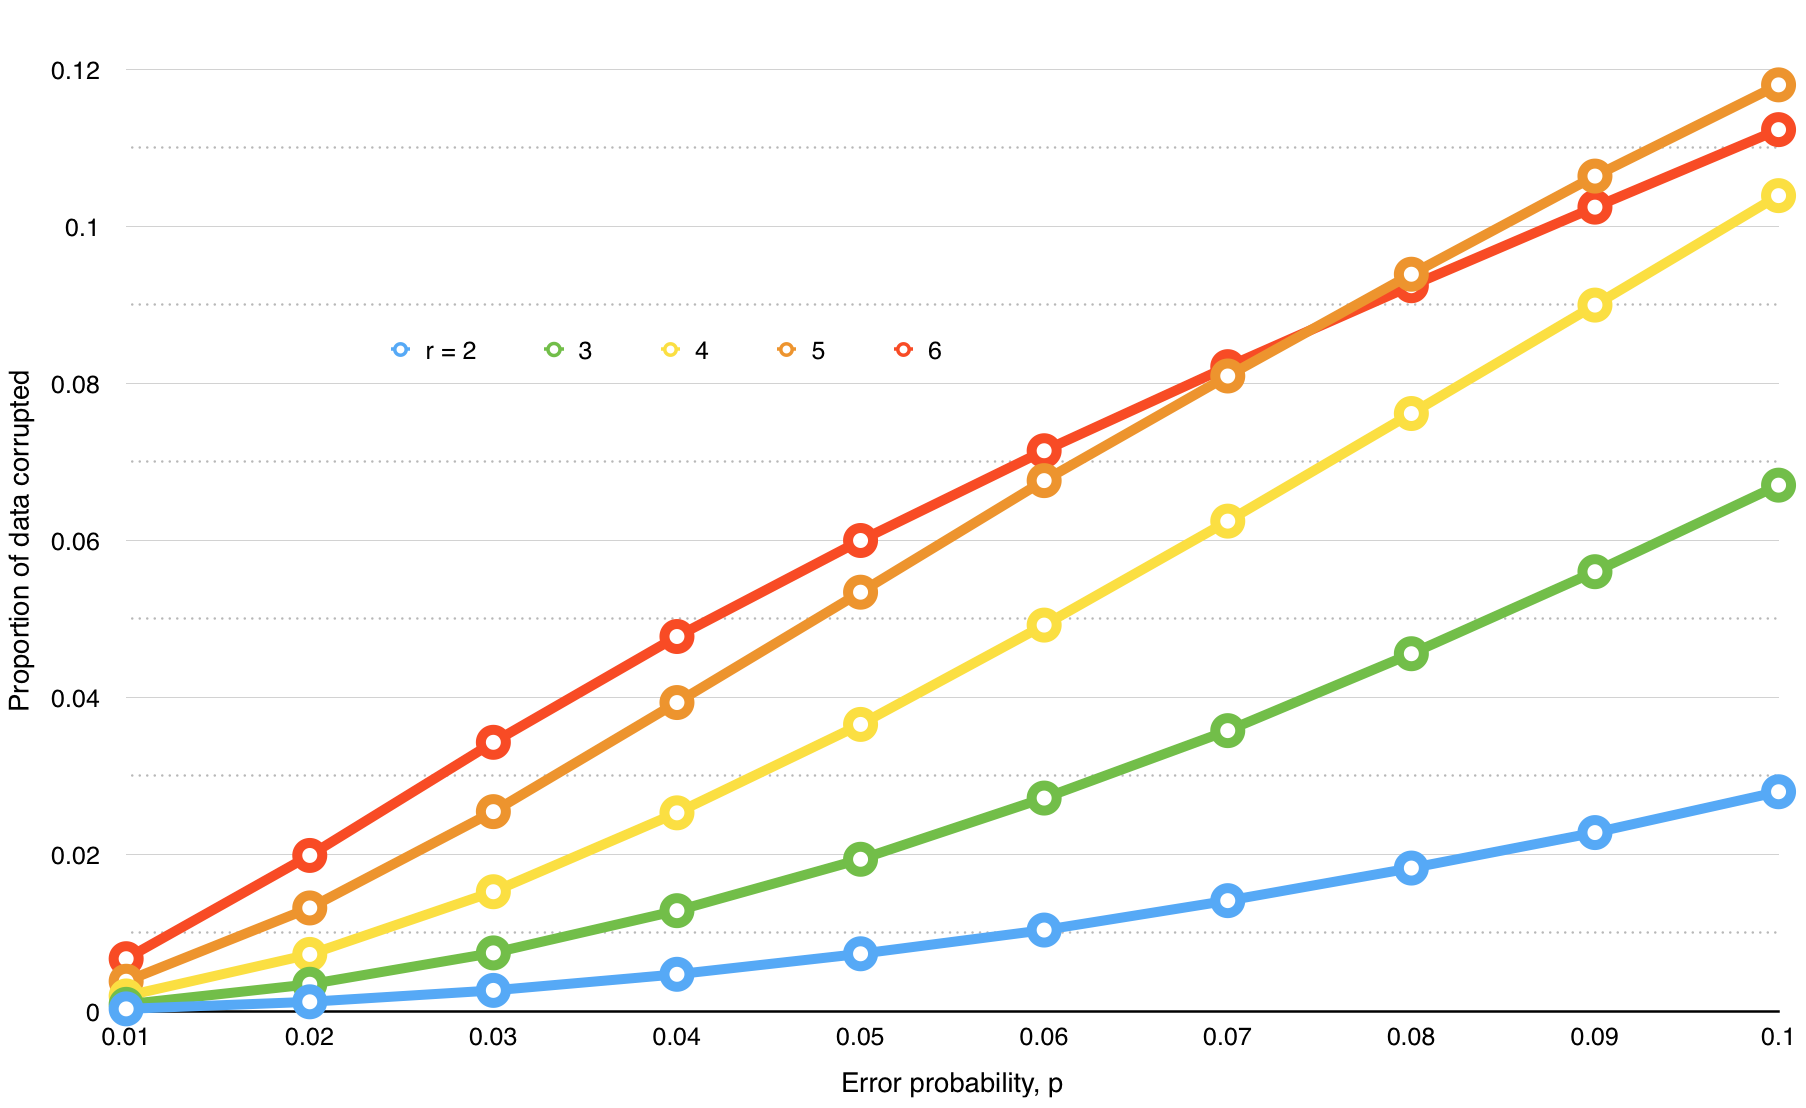
\includegraphics[width=\textwidth]{graph1}
        \end{figure}

        As shown in figure \ref{fig:graph1}, the trend of lower $r$ giving higher reliability as $p$ increases is very obvious, and the corruption increases exponentially as $p$ increases for low values of $r$. However, as we reach higher values of $r$, this exponential increase is no longer seen - for $r = 6$ the behaviour is more logarithmic, with the value of corruption greater than $p$ for all $p > 0.02$. To examine this more closely, we can look at a wider range of values for $p$.

        \begin{figure}[h]
            \caption{Error probability $p$ against data corruption for $r = 2..6$}
            \label{fig:graph2}
            \centering
            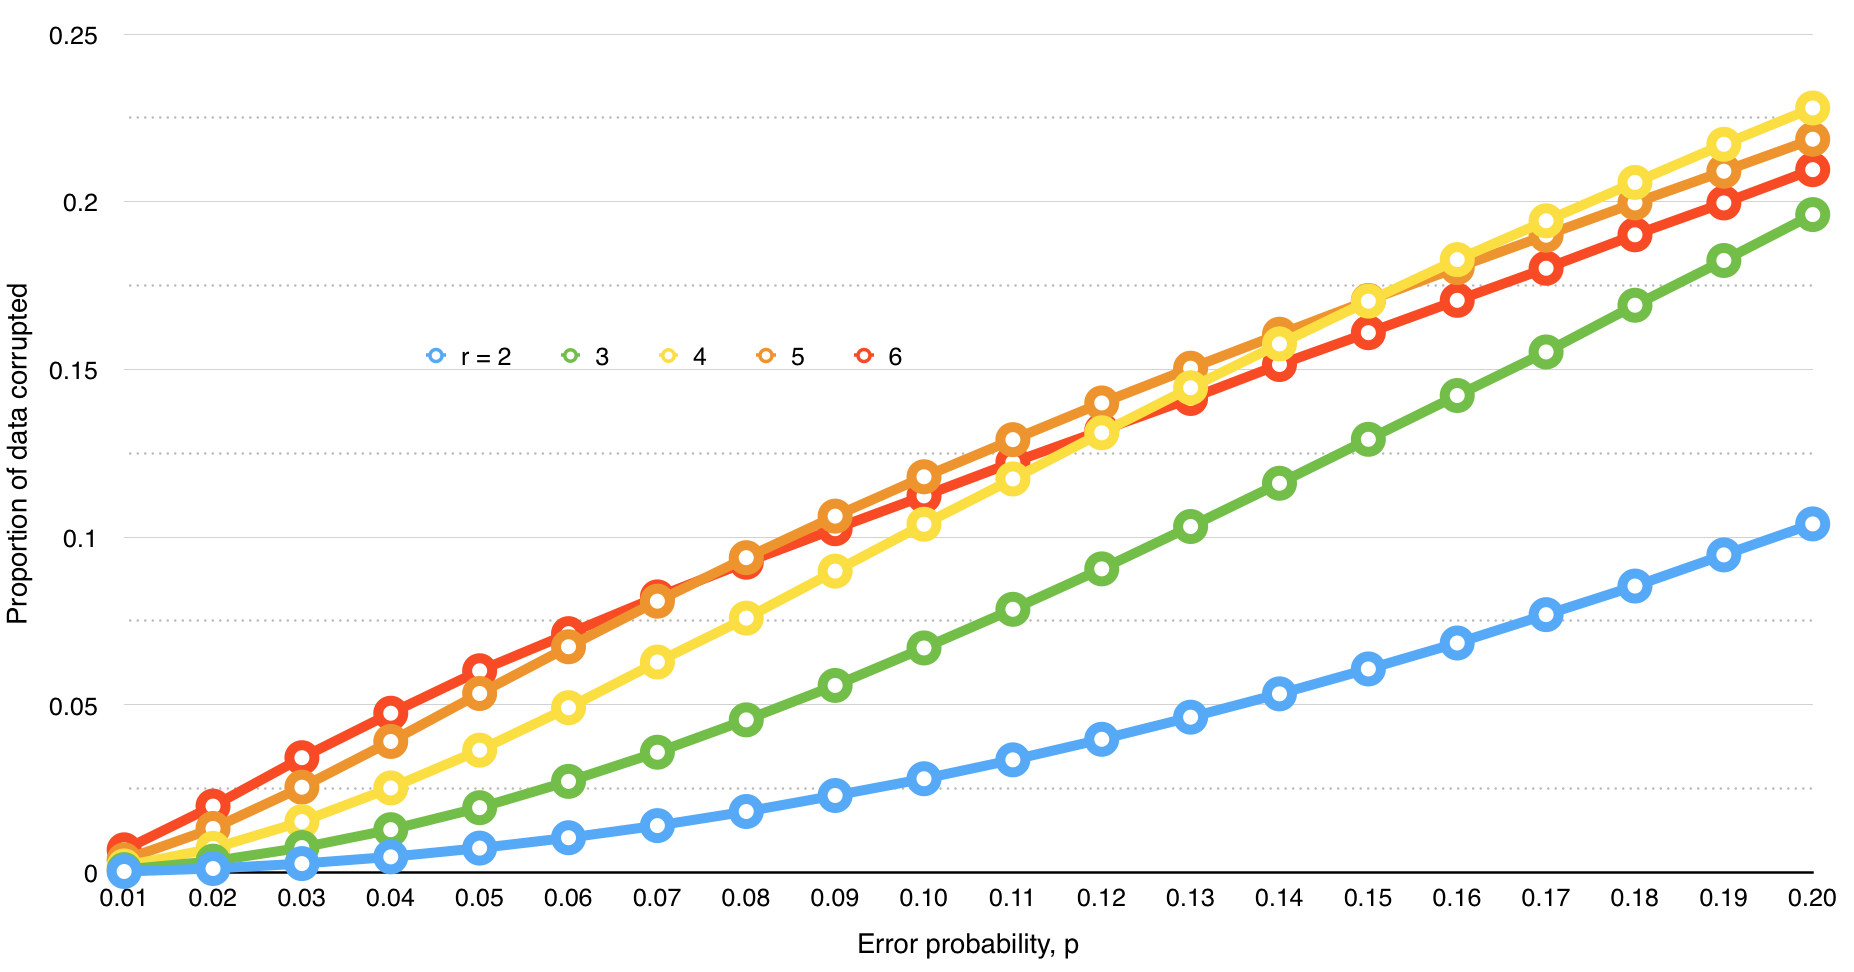
\includegraphics[width=\textwidth]{graph2}
        \end{figure}

        Figure \ref{fig:graph2} shows more clearly the logarithmic trend for other values of $r$. In particular, $r = 4$ now begins to show behaviour of both types - corruption increases exponentially until some point around $p = 0.10$ and then growth slows as it starts to tend to some value. The value of corruption at this point also seems to be around $0.10$ - level with $p$. This tends to imply that for all values of $r$, corruption will increase exponentially up until the point at which $p$ is equal to the corruption, from which growth will slow and tend to some value - which we can see from the previous tables is $p = 0.5$.

        So, from these two graphs (from data generated with the `-benchmark' flag) we can see that for any value of $r$, corruption increases exponentially with $p$ until the point at which $p$ is equal to the corruption, from which point corruption overtakes the error probability (i.e. the Hamming code is resulting in more errors than transmission alone) and then tends to 0.5 as $p$ tends to the same.

        \subsection{Crossover points}
            To try and find more information about where the crossover points occur for a given $r$ (i.e. for which values of $p$ a Hamming code is useful) a further program mode was created - running with the `-crossover' flag will calculate the corruption on a large, random data set for a starting value of $p$, then subtract/add half of the difference and continue to iterate in this manner until the two values have converged to within an acceptable range. This is obviously fairly imprecise, as the proportion of data corrupted is not reproducible for any given value of $p$ and the values will fluctuate. However, given enough time the program is able to converge on what seem to be fairly reasonable values for all values of $r$ from 2 to 11. ($r = 12$ was tried but due to time limitations could not be completed). Output from this benchmark may be seen below.

            \begin{verbatim}
r=2, p=0.4999183394197029
r=3, p=0.21130928123005022
r=4, p=0.09012692996053082
r=5, p=0.04198718085664379
r=6, p=0.020334432461346256
r=7, p=0.009987347877103469
r=8, p=0.004950081734557989
r=9, p=0.0024826915485493583
r=10, p=0.0012566530011336524
r=11, p=0.0006368131321779998
            \end{verbatim}

            From $r = 5$ and upwards, this seems to be very close to a geometric progression, halving at each interval (although less clear for the final few values as these were calculated with a larger accepted range to save time, so their accuracy is quite low). For $r = 5$ and upwards we can model this quite simply (and accurately) as $p=\frac{1}{25\times2^{(r - 5)}}$.

            Given this model, we are essentially able to calculate the optimum value of $r$ for a given value of $p$ in constant time (assuming $r < 0.4$). Given more work this model could definitely be improved.

\section{Building \& Execution}
    An \textit{ant} build file has been included with the source code. To build all source files, simply run \textit{\$ ant} with no arguments. Class files will be compiled to the `build' folder and a jar file will be created in the `dist' folder. Unit tests may be executed by running \textit{\$ ant test}.

    The program may be launched from the jar file in the standard way, e.g. \textit{\$ java -jar error-correction.jar}. When passing no arguments (or the `-h' flag), usage information will be printed.

\end{document}
